% {\small \textcolor{myblue}{Symposium on Molecular Simulations of Complex Fluids and Interfaces.}}

\vspace{-1em}

\begin{center}
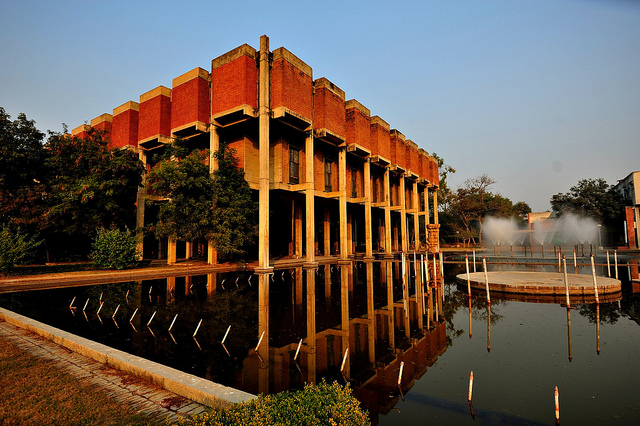
\includegraphics[width=0.6\textwidth]{images/lib.jpg}
\end{center}

\section{Welcome}

\vspace{-1em}

Welcome to the international symposium "Molecular Simulations of Complex Fluids and Interfaces", hosted at IIT Kanpur.

The behaviour of interfaces plays an important role in several industrial and natural processes. Molecular simulations can reveal microscopic insights into the structure and properties of solid-liquid interfaces. This meeting aims to provide a forum for exchanging ideas and sharing recent scientific advances from several perspectives. It is hoped that the current state of simulation methodologies will be established, paving the way for the future development of computational tools and research.

\vspace{-2em}

\section{Topics}

\vspace{-1em}

\begin{itemize}
  \itemsep-1em 
  \item Molecular Simulations: New Methodologies and Applications
  \item Advances in Coarse-Graining and Challenges
  \item Soft Matter Simulations
  \item Confined Fluids
  \item Wetting and Interfacial Phenomena
  \item Biomolecular Simulations
  \item Specific Systems and Models
\end{itemize}

% \pagebreak

% The following topics will be covered in the planned talks and lectures.



% \section{Organizing committee}
% \begin{center}
% \begin{tabular}{lll}
% Gloria Cecchini & Marco Faggian &  Aleksandra Pidde \\
% Rok Cestnik & R. Janis Goldschmidt &  Bastian Pietras\\
%  Pau Clusella  & Marc Grau Leguia & Eero Satuvuori \\
%  Nicolás Deschle & Maxime Lucas   &  Çağdaş Topçu \\
% Federico Devalle  & Irene Malvestio  & Clément Zankoc 
% \end{tabular}
% \end{center}